\documentclass[12pt,a4paper]{article}

% Packages
\usepackage[utf8]{inputenc}
\usepackage[T1]{fontenc}
\usepackage{geometry}
\usepackage{graphicx}
\usepackage{hyperref}
\usepackage{enumitem}
\usepackage{booktabs}
\usepackage{longtable}
\usepackage{fancyhdr}
\usepackage{titlesec}
\usepackage{caption}
\usepackage{subcaption}
\usepackage{listings}
\usepackage{xcolor}
\usepackage{amsmath}
\usepackage{tabularx}
\usepackage{array}
\usepackage{float}
\usepackage{tikz}
\usepackage{amssymb}
\usetikzlibrary{shapes.geometric, shapes.misc, arrows.meta, positioning, fit,
                backgrounds, calc, chains, decorations.pathreplacing}

\geometry{margin=2.5cm}

% ── Colours (for TikZ diagrams) ──────────────────────────────────────────────
\definecolor{clientblue}{RGB}{210,228,255}
\definecolor{gatewaygreen}{RGB}{210,240,220}
\definecolor{svcyellow}{RGB}{255,249,210}
\definecolor{dbgray}{RGB}{225,225,225}
\definecolor{mqorange}{RGB}{255,232,210}
\definecolor{redisred}{RGB}{255,218,218}
\definecolor{bordercolor}{RGB}{80,80,80}

% Header/Footer
\pagestyle{fancy}
\fancyhf{}
\fancyhead[L]{CS7NS6 -- Distributed Systems}
\fancyhead[R]{Exercise 2}
\fancyfoot[C]{\thepage}

% Hyperlink styling
\hypersetup{
    colorlinks=true,
    linkcolor=blue,
    citecolor=blue,
    urlcolor=blue
}

% Code listing style
\lstset{
    basicstyle=\ttfamily\small,
    breaklines=true,
    frame=single,
    backgroundcolor=\color{gray!10},
    keywordstyle=\color{blue},
    commentstyle=\color{green!50!black},
    stringstyle=\color{red!70!black}
}

% ── Table helpers ─────────────────────────────────────────────────────────────
\newcolumntype{L}[1]{>{\raggedright\arraybackslash}p{#1}}
\newcolumntype{C}[1]{>{\centering\arraybackslash}p{#1}}

% ── TikZ node styles ──────────────────────────────────────────────────────────
\tikzset{
  base/.style={draw=bordercolor, line width=0.7pt, align=center,
               font=\footnotesize, minimum height=0.85cm},
  client/.style   = {base, rounded corners=5pt, fill=clientblue,  minimum width=2.8cm},
  gateway/.style  = {base, rounded corners=5pt, fill=gatewaygreen, minimum width=5.2cm, minimum height=1.1cm},
  service/.style  = {base, rounded corners=4pt, fill=svcyellow,   minimum width=2.4cm},
  database/.style = {base, cylinder, shape border rotate=90, aspect=0.3,
                     fill=dbgray, minimum width=1.7cm, minimum height=0.9cm},
  broker/.style   = {base, rounded corners=4pt, fill=mqorange,    minimum width=2.4cm},
  cache/.style    = {base, cylinder, shape border rotate=90, aspect=0.3,
                     fill=redisred, minimum width=1.7cm, minimum height=0.9cm},
  arr/.style      = {-{Stealth[length=5pt]}, line width=0.7pt, color=bordercolor},
  darr/.style     = {-{Stealth[length=5pt]}, line width=0.6pt, dashed, color=bordercolor},
  lifeline/.style = {dashed, line width=0.5pt, color=bordercolor},
  msg/.style      = {-{Stealth[length=4pt]}, line width=0.6pt},
}

\begin{document}

% ============================================================
% TITLE PAGE
% ============================================================
\begin{titlepage}
    \centering
    \vspace*{1cm}

    \includegraphics[width=4cm]{tcd_logo.png}\\[1cm]

    {\Large \textbf{Trinity College Dublin}}\\[0.3cm]
    {\large School of Computer Science and Statistics}\\[2cm]

    {\LARGE \textbf{CS7NS6 -- Distributed Systems}}\\[0.5cm]
    {\Large 2025--2026}\\[1.5cm]

    {\Huge \textbf{Exercise 2:\\Implementing a Globally-accessible\\Distributed Service}}\\[2.5cm]

    {\Large \textbf{Group J\\[1.5cm]}

    \begin{tabular}{l l}
        \toprule
        \textbf{Name} & \textbf{Roll Number} \\
        \midrule
        Aditya Kumar Singh & 25340485 \\
        Parth Ashok Deshmukh & 25342469 \\
        Sai Eeshwar Divaakar & <Roll No.> \\
        Tanmay Ghosh & <Roll No.> \\
        Saurabh Deshmukh & <Roll No.> \\
        Sneha Meto & <Roll No.> \\
        \bottomrule
    \end{tabular}

    \vfill

    {\large \today}

\end{titlepage}

% ============================================================
% TABLE OF CONTENTS
% ============================================================
\newpage
\tableofcontents
\newpage

% ============================================================
% 1. INTRODUCTION
% ============================================================
\section{Introduction}

This project aims to create and engineer a \textbf{Globally Accessible Distribute Traffic System}. The system allows road-vehicle drivers to pre-book journeys before they travel. No driver may start a journey without a confirmed booking. The system checks for scheduling and road-capacity conflicts, notifies drivers of booking outcomes in real time via WebSocket, and allows roadside enforcement agents to verify active bookings instantly.
 
The system is composed of six independently deployable services as User Service, Journey Service, Conflict Service, Notification Service, Enforcement Service, and Analytics Service. Each service has its own database, and communicates via both synchronous REST calls and asynchronous messaging through RabbitMQ. The infrastructure includes PostGres streaming replication, Redis Sentinel for high availability, HAProxy load balancing, and nginx API gateway rate limiting.
 
The remainder of this report is organised as follows: Section~\ref{sec:requirements} describes the functional and non-functional requirements; Section~\ref{sec:specification} provides a detailed specification of services and APIs; Section~\ref{sec:architecture} covers the system architecture and individual service designs; Section~\ref{sec:implementation} details key algorithms and failure handling; Section~\ref{sec:testing} outlines the test plan and results; Section~\ref{sec:allocation} describes the allocation of work; and Section~\ref{sec:conclusion} summarises the achievements of the project.

% ============================================================
% 2. REQUIREMENTS
% ============================================================
\section{Requirements}
\label{sec:requirements}
 
\subsection{System Overview}
 
The Journey Booking System provides a platform for road-vehicle drivers to create, manage, and cancel journey bookings. The system enforces that no driver may begin a journey without a confirmed booking. It detects scheduling conflicts (overlapping driver or vehicle bookings and road-segment capacity limits), delivers real-time notifications, and exposes an enforcement verification interface for roadside agents.
 
\subsection{Functional Requirements}
 
The system addresses the following functional requirements:
 
\begin{enumerate}[label=\textbf{FR\arabic*}]
    \item \textbf{User Registration and Authentication:} Drivers and enforcement agents can register accounts and authenticate via JWT tokens. Passwords are hashed with bcrypt. Separate \texttt{DRIVER} and \texttt{ENFORCEMENT\_AGENT} roles are supported. Vehicle registration is linked to user accounts.
    \item \textbf{Journey Booking:} Drivers can create journey bookings specifying origin, destination (with coordinates), departure time, estimated duration, and vehicle registration. Bookings are confirmed only after passing conflict checks. The system returns \texttt{CONFIRMED} or \texttt{REJECTED} with a reason.
    \item \textbf{Conflict Detection:} The system checks for three types of conflicts before confirming a booking: driver overlap (same driver has an overlapping confirmed journey), vehicle overlap (same vehicle already booked), and road-segment capacity (grid cell at maximum capacity for the time slot).
    \item \textbf{Journey Cancellation:} Drivers can cancel their own bookings. Cancellation releases reserved road capacity, removes enforcement cache entries, and notifies all downstream services via event fan-out.
    \item \textbf{Real-time Notifications:} Drivers receive push notifications via WebSocket for booking confirmations, rejections, and cancellations. A notification history endpoint provides the last 50 entries with a 7-day TTL.
    \item \textbf{Enforcement Verification:} Enforcement agents can verify whether a vehicle or driver holds an active booking by querying by vehicle plate or driving licence number with sub-second response times.
    \item \textbf{Analytics and Monitoring:} The system records journey events, provides real-time statistics, hourly aggregated reports, and an aggregated health view of all services.
    \item \textbf{Points System:} Each confirmed journey earns the driver points based on distance and duration, tracked via a pessimistically locked points ledger.
    \item \textbf{Idempotent Retries:} Clients supply an \texttt{Idempotency-Key} header; duplicate booking requests return the cached result without re-running the saga.
\end{enumerate}
 
\subsection{Non-Functional Requirements}
\label{sec:nfr}
 
\begin{table}[H]
\centering\small
\begin{tabularx}{\textwidth}{L{3.2cm} L{4.4cm} X}
  \toprule
  \textbf{Property} & \textbf{Target} & \textbf{Rationale / Mechanism} \\
  \midrule
  Availability & $\geq 99.5\%$ under a single node failure & Active-active
        deployment: clients transparently fail over to a surviving node
        through the browser's \texttt{resilientFetch} layer. \\\addlinespace[0.1cm]
  Booking latency & $<400\,$ms at p95 under normal load & End-to-end saga
        (journey row $\to$ conflict check $\to$ outbox) benchmarks at
        100--250\,ms on the slim stack. \\\addlinespace[0.1cm]
  Enforcement latency & $<200\,$ms hard limit (cache hit $<20\,$ms p95) &
        Redis-first lookup with a journey-service fallback path. \\\addlinespace[0.1cm]
  Consistency & Strong per-slot (no double booking) & \texttt{SERIALIZABLE}
        transaction with \texttt{SELECT FOR UPDATE} inside the conflict
        service. \\\addlinespace[0.1cm]
  Eventual consistency & Cross-service state converges after a partition
        heals & Transactional outbox $+$ at-least-once RabbitMQ delivery,
        idempotent consumers. \\\addlinespace[0.1cm]
  Durability & No confirmed booking is ever lost & Event stored in the same
        DB transaction as the journey row; background drainer replays to
        RabbitMQ after broker recovery. \\\addlinespace[0.1cm]
  Fault Tolerance & System degrades, does not crash & Transactional outbox pattern, circuit breakers, Redis Sentinel, and Postgres streaming replication. When the conflict service is unreachable, the circuit breaker opens and bookings fail fast rather than hanging. When infrastructure peers are down, the system enters \texttt{LOCAL\_ONLY} mode. \\\addlinespace[0.1cm]
  Partition tolerance & System degrades gracefully & Partition manager
        per service (CONNECTED $\to$ SUSPECTED $\to$ PARTITIONED $\to$
        MERGING). Circuit breaker fails fast on dependency outage. \\\addlinespace[0.1cm]
  Scalability & Independent service scaling & The microservices architecture allows independent scaling of services. Read/write separation via PostGres replicas offloads read traffic. \\\addlinespace[0.1cm]
  Idempotency & No duplicate side effects & Duplicate booking requests (same idempotency key) return cached results. Message consumers deduplicate via Redis \texttt{SETNX} on message IDs. \\\addlinespace[0.1cm]
  Observability & All cross-service calls traceable & \texttt{X-Request-ID}
        propagated; \texttt{X-Partition-Status} and
        \texttt{X-Cache-Stale} headers exposed on responses. \\
  \bottomrule
\end{tabularx}
\caption{Non-functional requirements}
\label{tab:nfr}
\end{table}

\subsection{Failure Model}

We adopt a \textbf{crash-recovery} failure model with asynchronous network. Services may crash and restart at any time; all durable state lives in PostgreSQL, RabbitMQ or Redis. Messages between services may be delayed, duplicated or lost. We assume a trusted internal network between services, so Byzantine faults are out of scope. Correlated failures are mitigated by running the full stack on each participating node so that losing one laptop does not take the system down.

% ============================================================
% 3. SPECIFICATION
% ============================================================
\section{Specification}
\label{sec:specification}
 
\subsection{System Services}
 
The system is composed of six independent microservices, each with its own Postgres database:
 
\begin{table}[H]
\centering\small
\begin{tabularx}{\textwidth}{L{2.7cm} L{1.4cm} L{2.6cm} X}
  \toprule
  \textbf{Service} & \textbf{Lang / Port} & \textbf{Data store} & \textbf{Responsibility} \\
  \midrule
  User          & Py / 8001 & Postgres \texttt{users\_db} + replica &
      Registration, login (JWT), vehicle CRUD. Publishes
      \texttt{user.registered}. Routes reads to replica, writes to primary. \\\addlinespace[0.1cm]
  Journey       & Py / 8002 & Postgres \texttt{journeys\_db} + replica &
      Booking saga orchestration, idempotency, outbox drainer, circuit
      breaker, lifecycle scheduler, partition detector, 2PC coordinator,
      peer health model. \\\addlinespace[0.1cm]
  Conflict      & Go / 8003 & Postgres \texttt{conflicts\_db} + replica &
      Atomic capacity check (\texttt{SERIALIZABLE} + \texttt{SELECT FOR UPDATE}),
      grid-cell road model ($\approx$ 0.01\textdegree, approximately 1\,km per cell, 30-minute time slots), REST slot replication to peer nodes, idempotent
      cancellation consumer. \\\addlinespace[0.1cm]
  Notification  & Go / 8004 & Redis &
      WebSocket push, consumer deduplication via Redis \texttt{SETNX},
      notification history (7-day TTL, 50 entries/user), DLQ,
      auto-reconnect. \\\addlinespace[0.1cm]
  Enforcement   & Py / 8005 & Redis + journey API &
      Redis-first lookup; licence$\to$user id cache (24\,h TTL);
      event-driven invalidation; \texttt{X-Cache-Stale} header on
      partition. \\\addlinespace[0.1cm]
  Analytics     & Go / 8006 & Postgres \texttt{analytics\_db} + replica + Redis &
      Dual-write counters, hourly roll-up goroutine, replica-lag endpoint,
      aggregated service health. \\
  \bottomrule
\end{tabularx}
\caption{Service inventory}
\label{tab:services}
\end{table}

\subsection{Service APIs}

All external traffic enters through HAProxy $\to$ two nginx gateway instances. nginx applies three rate-limit zones (\texttt{auth}: 5\,r/m, \texttt{booking}: 30\,r/m, \texttt{general}: 60\,r/m) and routes to the owning service. Table~\ref{tab:api} lists APIs by service.



\begin{table}[H]
\centering
\scriptsize
\setlength{\tabcolsep}{3pt}
\begin{tabularx}{\textwidth}{L{1.6cm} @{\hspace{6pt}} L{1.1cm} @{\hspace{6pt}} L{6.2cm} @{\hspace{6pt}} X}
  \toprule
  \textbf{Service} & \textbf{Method} & \textbf{Path} & \textbf{Description} \\
  \midrule
 
  %% ── User Service ──────────────────────────────────────────────────
  User (Python)
    & GET    & \texttt{/api/users/me}                                       & Current user's profile \\
    & GET    & \texttt{/api/users/license/\{license\_number\}}              & Look up user by licence number \\
    & GET    & \texttt{/api/users/vehicles}                                 & List current user's vehicles \\
    & GET    & \texttt{/api/users/vehicles/verify/\{registration\}}         & Verify vehicle ownership \\
    & POST   & \texttt{/api/users/register}                                 & Register a driver account \\
    & POST   & \texttt{/api/users/register/agent}                           & Register an enforcement agent account \\
    & POST   & \texttt{/api/users/login}                                    & Login, returns JWT token \\
    & POST   & \texttt{/api/users/vehicles}                                 & Register a vehicle \\
    & DELETE & \texttt{/api/users/vehicles/\{vehicle\_id\}}                 & Remove a vehicle \\
  \midrule
 
  %% ── Journey Service ───────────────────────────────────────────────
  Journey (Python)
    & GET    & \texttt{/api/journeys/}                                      & List current user's journeys \\
    & GET    & \texttt{/api/journeys/all}                                   & Admin: all journeys across all users \\
    & GET    & \texttt{/api/journeys/\{journey\_id\}}                       & Get a specific journey \\
    & GET    & \texttt{/api/journeys/points/balance}                        & Current user's points balance \\
    & GET    & \texttt{/api/journeys/points/history}                        & Points transaction history \\
    & GET    & \texttt{/api/journeys/vehicle/\{vehicle\_reg\}/active}       & Active journeys for a vehicle \\
    & GET    & \texttt{/api/journeys/user/\{user\_id\}/active}              & Active journeys for a user \\
    & POST   & \texttt{/api/journeys/} (\texttt{?mode=2pc})                 & Book a journey (saga / Two-Phase Commit) \\
    & POST   & \texttt{/api/journeys/points/spend}                          & Spend points (\texttt{?amount=}) \\
    & DELETE & \texttt{/api/journeys/\{journey\_id\}}                       & Cancel a journey \\
  \midrule
 
  %% ── Conflict Service ──────────────────────────────────────────────
  Conflict (Go)
    & GET    & \texttt{/api/routes}                                         & List all road routes \\
    & GET    & \texttt{/api/conflicts/routes}                               & Same as above (alternate nginx prefix) \\
    & POST   & \texttt{/api/conflicts/check}                                & Check capacity conflicts before booking \\
    & POST   & \texttt{/api/conflicts/cancel/\{journey\_id\}}               & Cancel a booking slot (frees capacity) \\
  \midrule
 
  %% ── Enforcement Service ───────────────────────────────────────────
  Enforcement (Python)
    & GET    & \texttt{/api/enforcement/verify/vehicle/\{reg\}}    & Verify vehicle has active booking (agent only) \\
    & GET    & \texttt{/api/enforcement/verify/license/\{lic\_no\}} & Verify driver by licence number (agent only) \\
  \midrule
 
  %% ── Notification Service ──────────────────────────────────────────
  Notification (Go)
    & GET    & \texttt{/api/notifications/}                                 & Get notifications (\texttt{?token=}, \texttt{?limit=}) \\
    & WS     & \texttt{/ws/notifications/}                                  & WebSocket stream of real-time notifications (\texttt{?token=}) \\
  \midrule
 
  %% ── Analytics Service ─────────────────────────────────────────────
  Analytics (Go)
    & GET    & \texttt{/api/analytics/stats}                                & System-wide booking stats \\
    & GET    & \texttt{/api/analytics/events}                               & Event history (\texttt{?event\_type=}, \texttt{?limit=}, \texttt{?offset=}) \\
    & GET    & \texttt{/api/analytics/hourly}                               & Hourly booking stats (\texttt{?limit=}, max 168h) \\
    & GET    & \texttt{/api/analytics/replica-lag}                          & PostgreSQL replication lag (\texttt{pg\_stat\_replication}) \\
    & GET    & \texttt{/api/analytics/health/services}                      & Aggregate health check of all 6 services \\
  \midrule
 
  %% ── Health / Admin (cross-service) ────────────────────────────────
  All services
    & GET    & \texttt{/health}                                             & Health check (503 when node simulated-failed) \\
    & GET    & \texttt{/health/partitions}                                  & Partition status of dependencies \\
    & GET    & \texttt{/health/nodes}                                       & Per-peer ALIVE / SUSPECT / DEAD status \\
    & GET    & \texttt{/admin/logs}                                         & Recent log entries (ring buffer) \\
    & GET    & \texttt{/admin/simulate/status}                              & Current simulation state \\
    & POST   & \texttt{/admin/simulate/fail}                                & Simulate node crash (cascades to user-service) \\
    & POST   & \texttt{/admin/simulate/recover}                             & Recover from simulated failure \\
    & POST   & \texttt{/admin/peers/register}                               & Register a remote peer to monitor \\
    & POST   & \texttt{/admin/recovery/drain-outbox}                        & Force-drain unpublished outbox events \\
    & POST   & \texttt{/admin/recovery/rebuild-enforcement-cache}           & Rebuild enforcement Redis cache from DB \\
    & POST   & \texttt{/admin/2pc/demo}                                     & Info on triggering 2PC demo \\
    & DELETE & \texttt{/admin/peers/\{name\}}                               & Unregister a peer \\
  \bottomrule
\end{tabularx}
\caption{Full API surface across all six microservices}
\end{table}

\subsection{Internal APIs and Events}

Two additional interfaces exist purely between services:

\begin{itemize}
  \item \textbf{REST (south-bound):} \texttt{POST /api/conflicts/check}
        (journey $\to$ conflict, reserves a slot inside a serialisable
        transaction), \texttt{POST /api/conflicts/cancel/\{id\}}
        (compensating call used by the 2PC coordinator), and the
        \texttt{/internal/slots/*} family used for cross-node slot
        replication (see Section~\ref{sec:replication}).
  \item \textbf{RabbitMQ topic exchange} \texttt{journey\_events}:
        \texttt{user.registered}, \texttt{journey.confirmed},
        \texttt{journey.rejected}, \texttt{journey.cancelled},
        \texttt{journey.completed}. Each consumer queue has its own DLX
        with 24\,h TTL.
\end{itemize}

\subsection{Fault Behaviour}
 
The system is designed to handle the following fault scenarios. Table~\ref{tab:faults} captures how the system responds to each important failure class.

\begin{table}[H]
\centering\footnotesize
\begin{tabularx}{\textwidth}{L{3.4cm} X X}
  \toprule
  \textbf{Fault} & \textbf{System behaviour} & \textbf{Guarantee retained} \\
  \midrule
  Journey service crash &
    HAProxy+nginx mark backend unhealthy; in-flight requests fail. Outbox
    drainer resumes on restart. Browser \texttt{resilientFetch} retries
    peer. &
    No confirmed booking lost; idempotency prevents duplicates on retry. \\\addlinespace[0.1cm]
  Conflict service crash &
    Circuit breaker opens after three consecutive failures; subsequent
    bookings fail instantly with a clear error. &
    Failures are bounded, system does not hang; booking attempts can
    always be retried. \\\addlinespace[0.1cm]
  RabbitMQ outage &
    Outbox row is written in the same transaction as the journey;
    background drainer replays on reconnect. Consumers auto-reconnect. &
    At-least-once publication and delivery; eventual consistency of
    downstream state. \\\addlinespace[0.1cm]
  Redis primary loss &
    Sentinel-based failover promotes replica; services reconnect via
    \texttt{REDIS\_SENTINEL\_ADDRS}. Enforcement service transparently
    continues. & Cache availability, bounded staleness. \\\addlinespace[0.1cm]
  Postgres replica lag &
    Reads continue against the primary; lag visible at
    \texttt{/api/analytics/replica-lag}. & Read availability. \\\addlinespace[0.1cm]
  Network partition between nodes &
    Each node's conflict service rejects bookings inside its local
    partition set; replication back-fills after merge via a 5-minute
    re-sync goroutine plus catch-up sync on peer register. & No local
    double bookings; eventual global convergence. \\\addlinespace[0.1cm]
  Full-node kill (simulated) &
    Journey + user services set \texttt{\_node\_failed=True}; all routes
    return 503 except \texttt{/health} and the simulate endpoints.
    Browser fails over to peer transparently. & Session preserved via
    cross-node JWT secret; peer-list persisted to localStorage. \\\addlinespace[0.1cm]
  Peer node failure &
    ALIVE/SUSPECT/DEAD health model detects unresponsive peers. After 3 missed
    health checks, a peer transitions to SUSPECT; after 6, to DEAD. If fewer
    than 50\% of peers are alive, the system enters \texttt{LOCAL\_ONLY} mode. & Graceful degradation. \\\addlinespace[0.1cm]
  Message redelivery &
    All consumers implement deduplication. Notification and Analytics services use Redis \texttt{SETNX} on message IDs (24-hour TTL). Conflict Service cancellation consumer is idempotent---redelivered events find \texttt{is\_active = false} and are acknowledged silently. & Effectively-exactly-once processing. \\\addlinespace[0.1cm]
  \textbf{Not fully addressed} &
    Saga compensation on conflict-service failure is not retried;
    HMAC audit chain incomplete; enforcement cache cold on startup;
    token blacklist on logout absent; 3-node RabbitMQ cluster unreliable
    on a single Docker host. & --- \\
  \bottomrule
\end{tabularx}
\caption{Fault-handling matrix}
\label{tab:faults}
\end{table}

\subsection{Limitations and Unaddressed Requirements}
 
The following limitations are known and documented for consistency with the demonstration:
 
\begin{itemize}
    \item \textbf{Saga compensating transactions:} If the Conflict Service is down during a booking attempt, the saga rejects the booking permanently with no retry or compensating transaction.
    \item \textbf{Audit HMAC chain:} The \texttt{event\_logs} table records a full event history with timestamps, but the planned cryptographic integrity chain (HMAC) was not completed.
    \item \textbf{WebSocket registry:} The Notification Service's WebSocket connection registry is held in memory only and is lost on service restart.
    \item \textbf{Enforcement cache cold start:} After startup, the first enforcement request always misses the Redis cache; there is no cache warming on boot.
    \item \textbf{Token blacklisting:} Revoked JWT tokens remain valid until their natural expiry; no token blacklist is implemented.
    \item \textbf{RabbitMQ clustering:} A 3-node RabbitMQ cluster is configured, but Erlang distribution is unreliable on a single Docker host. The single-node deployment demonstrates all messaging principles.
    \item \textbf{Distributed tracing visualisation:} Correlation IDs (\texttt{X-Request-ID}) are propagated across all services, but no span visualisation tool (e.g., Jaeger or Zipkin) is integrated.
\end{itemize}

% ============================================================
% 4. ARCHITECTURE AND DESIGN
% ============================================================
\section{Architecture and Design}
\label{sec:architecture}
 
\subsection{System Architecture}
 \begin{figure}[H]
    \centering
    \includegraphics[width=1\textwidth]{newarch.png}
    \caption{System architecture.}
\end{figure}
The system follows a microservices architecture with six independently deployable services. Client requests enter through HAProxy (port 8080), which load-balances across two nginx API gateway instances. Nginx enforces rate limiting in three zones (authentication at 5\,req/min, booking at 30\,req/min, and general at 60\,req/min) and routes requests to the appropriate service based on URL prefix.
 
Each service owns its data exclusively and thus, there are no shared databases. Services communicate synchronously via REST (the Journey Service calls the Conflict Service during the saga) and asynchronously via RabbitMQ using a topic exchange (\texttt{journey\_events}) with routing keys per event type (e.g., \texttt{journey.confirmed}, \texttt{journey.cancelled}).

In multi-node mode (the distinguishing feature of branch \texttt{approach3}), the \emph{entire stack} runs on every participating laptop. Nodes learn about each other through the \texttt{PEER\_CONFLICT\_URLS} and \texttt{PEER\_USER\_URLS} environment variables and through runtime registration at \texttt{/admin/peers/register}. Slot state is replicated between conflict services over REST; health is tracked with an ALIVE/SUSPECT/DEAD state machine; clients fail over between nodes through a JavaScript \texttt{resilientFetch} wrapper.

\begin{figure}[H]
\centering
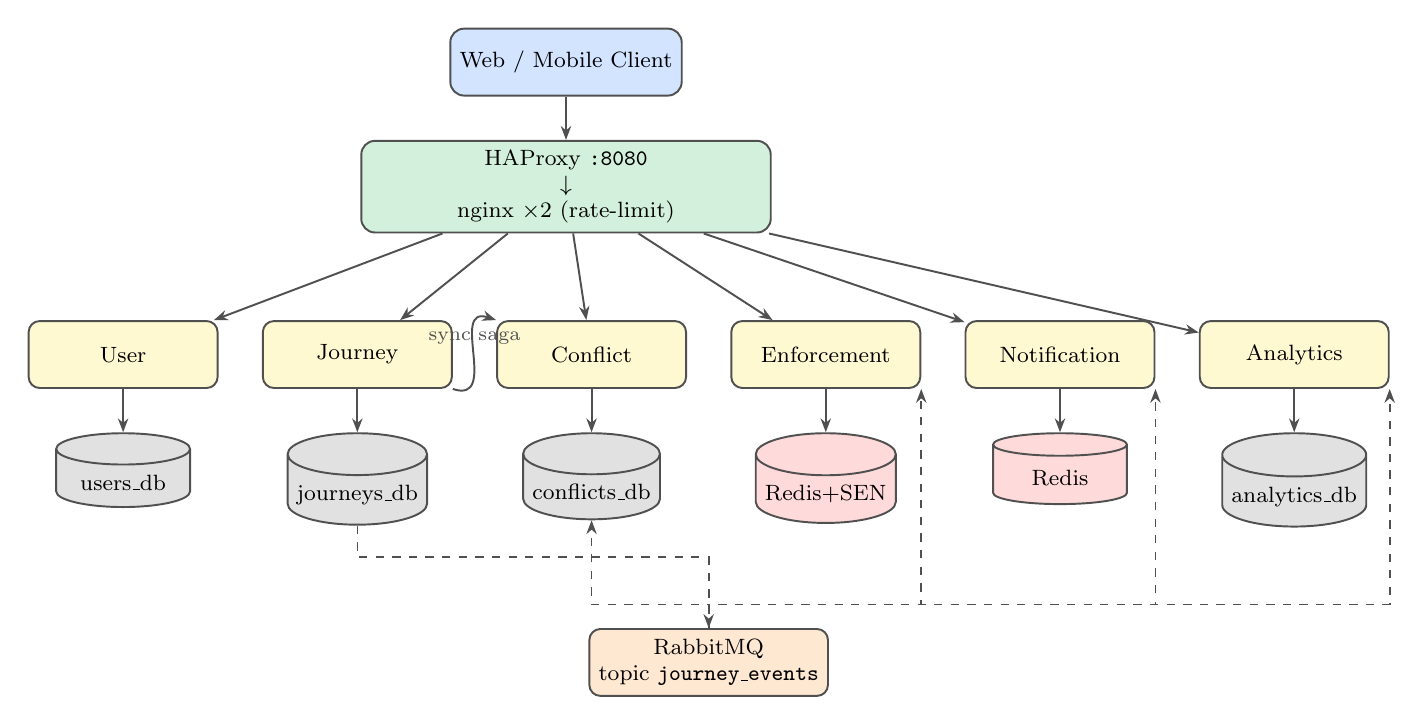
\begin{tikzpicture}[node distance=0.55cm and 0.55cm]
  \node[client] (client) {Web / Mobile Client};
  \node[gateway, below=of client] (gw)
       {HAProxy \texttt{:8080} \\ $\downarrow$ \\ nginx $\times 2$ (rate-limit)};
  \node[service, below left=1.1cm and 1.8cm of gw] (user)  {User};
  \node[service, right=of user]                     (jrny)  {Journey};
  \node[service, right=of jrny]                     (cnf)   {Conflict};
  \node[service, right=of cnf]                      (enf)   {Enforcement};
  \node[service, right=of enf]                      (notif) {Notification};
  \node[service, right=of notif]                    (anl)   {Analytics};
  \node[database, below=of user]  (udb)  {users\_db};
  \node[database, below=of jrny]  (jdb)  {journeys\_db};
  \node[database, below=of cnf]   (cdb)  {conflicts\_db};
  \node[cache,    below=of enf]   (rds)  {Redis+SEN};
  \node[cache,    below=of notif] (nrd)  {Redis};
  \node[database, below=of anl]   (adb)  {analytics\_db};

  % Centre RabbitMQ below the database row, midpoint of all services
  \path (udb.south) -- (adb.south) coordinate[midway] (dbmid);
  \node[broker, below=1.4cm of dbmid] (mq) {RabbitMQ \\ topic \texttt{journey\_events}};

  \draw[arr] (client)--(gw);
  \foreach \s in {user,jrny,cnf,enf,notif,anl} \draw[arr] (gw)--(\s);
  \draw[arr] (user)--(udb);
  \draw[arr] (jrny)--(jdb);
  \draw[arr] (cnf)--(cdb);
  \draw[arr] (anl)--(adb);
  \draw[arr] (enf)--(rds);
  \draw[arr] (notif)--(nrd);
  \draw[arr] (jrny.south east) .. controls +(0.6,-0.2) and +(-0.6,0.2) .. (cnf.north west)
        node[midway,above,font=\scriptsize]{sync saga};
  \draw[darr] (jdb.south) -- ++(0,-0.4) -| (mq);
  \draw[darr] (mq.north) -- ++(0,0.3) -| (notif.south east);
  \draw[darr] (mq.north) -- ++(0,0.3) -| (enf.south east);
  \draw[darr] (mq.north) -- ++(0,0.3) -| (anl.south east);
  \draw[darr] (mq.north) -- ++(0,0.3) -| (cdb.south);
\end{tikzpicture}
\caption{High-level runtime topology. Solid arrows are synchronous REST;
dashed arrows are asynchronous RabbitMQ events. Each service owns its
database; Redis+Sentinel backs enforcement, notification and analytics.}
\label{fig:architecture}
\end{figure}

\textbf{Request path for journey booking:}
 
\begin{enumerate}
    \item Client sends \texttt{POST /api/journeys/} with an \texttt{Idempotency-Key} header.
    \item Nginx routes the request to the Journey Service.
    \item Journey Service creates a journey row in \texttt{PENDING} state.
    \item Journey Service calls Conflict Service (\texttt{POST /api/conflicts/check}) synchronously.
    \item Conflict Service executes a \texttt{SERIALIZABLE} transaction with \texttt{SELECT FOR UPDATE}, checking driver overlap, vehicle overlap, and road capacity.
    \item If approved: Journey Service writes the journey row (status \texttt{CONFIRMED}) and an outbox event in the same database transaction.
    \item Background thread drains the outbox to RabbitMQ.
    \item Downstream consumers receive the event: Notification Service pushes via WebSocket, Analytics Service increments counters, Enforcement Service caches the active journey in Redis.
\end{enumerate}
 
\subsection{Software Architecture}
 
The services are implemented in two languages: Python (User, Journey, Enforcement) and Go (Conflict, Notification, Analytics). Shared Python modules provide cross-cutting concerns:
 
\begin{itemize}
    \item \texttt{shared/circuit\_breaker.py}: circuit breaker with configurable failure threshold and recovery timeout (closed/open/half-open states).
    \item \texttt{shared/partition.py}: partition detection state machine probing Postgres, RabbitMQ, and upstream services every 5\,s.
    \item \texttt{shared/tracing.py}: correlation ID generation and propagation via \texttt{X-Request-ID} headers with structured logging.
    \item \texttt{shared/rabbitmq.py}: durable publishers/consumers with reconnect, DLX wiring and consumer deduplication helper.
\end{itemize}

Go services (conflict, notification, analytics) use small hand-written packages for the same concerns rather than a shared module.
 
Infrastructure is containerised using Docker Compose. The full stack comprises up to 26 containers (6 services, 8 Postgres instances, 2 Redis instances, 3 Sentinel instances, 3 RabbitMQ nodes, 2 nginx instances, 1 HAProxy, and 1 frontend). A slim deployment profile reduces this to 12 containers for resource-constrained environments.
 
\subsection{Runtime Services and Distribution}
 
At runtime, the following infrastructure services support the application:
 
\begin{itemize}
    \item \textbf{Postgres} (4 primary--replica pairs): WAL streaming replication. Each service database has its own primary and replica. Replicas are initialised via \texttt{pg\_basebackup}.
    \item \textbf{Redis} (primary + replica + 3 Sentinels): Used for enforcement caching, notification history, analytics counters, and consumer deduplication keys. Sentinel provides automatic failover with a quorum of 2.
    \item \textbf{RabbitMQ}: Topic exchange \texttt{journey\_events} with per-consumer queues. Dead-letter exchanges (DLX) and dead-letter queues (DLQ) are configured per consumer with 24-hour TTL.
    \item \textbf{HAProxy + nginx}: HAProxy fronts two nginx instances. Nginx handles rate limiting and upstream routing to services.
\end{itemize}
 
\subsection{Individual Service Designs}
 
Each team member was responsible for the design of one or more services. The following subsections describe the most significant service each member contributed.
 
\subsubsection{User Service: Parth Deshmukh}
 
The User Service provides stateless JWT-based authentication and serves as the entry point for driver and enforcement agent registration. It routes read queries to a Postgres streaming replica and write queries to the primary, implementing read/write separation at the application level via a \texttt{Session.get\_bind()} override at the SQLAlchemy level.
 
On successful registration, the service publishes a \texttt{user.registered} event to RabbitMQ, making it a full participant in the event bus. Vehicle registration is linked to user accounts and is required before a driver can book a journey. JWTs are signed with a shared secret across nodes, which allows the browser to re-use a session on the failover peer without a re-login.

During a simulated node kill, the service installs an HTTP middleware that returns 503 for every path except \texttt{/health}, \texttt{/admin/simulate/fail} and \texttt{/admin/simulate/recover}, so from a peer's point of view the entire user-facing surface of the node disappears at once.

A known limitation is that no token blacklisting is implemented on logout, so revoked JWTs remain valid until their natural expiry.
 
\subsubsection{Journey Service: Tanmay Ghosh}
 
The Journey Service is the most architecturally complex service in the system, serving as the saga orchestrator. Its design centres on several distributed systems patterns:
 
The \textbf{transactional outbox} ensures that journey state changes and their corresponding events are written atomically in a single database transaction to the \texttt{journey\_events} table. A background thread polls this table and drains unpublished events to RabbitMQ, guaranteeing at-least-once delivery even if the broker is temporarily unavailable. Coupling the domain write to the event write eliminates the dual-write problem (``wrote to DB, crashed before publish'') without needing a distributed transaction.
 
The \textbf{circuit breaker} wraps the synchronous REST call to the Conflict Service. It tracks consecutive failures and, after a configurable threshold (default: 3), opens the circuit so that subsequent booking requests fail immediately rather than accumulating timeouts.
 
The \textbf{partition detection} module probes Postgres, RabbitMQ, and the Conflict Service every 5 seconds, transitioning through \texttt{CONNECTED} $\rightarrow$ \texttt{SUSPECTED} $\rightarrow$ \texttt{PARTITIONED} $\rightarrow$ \texttt{MERGING} states. The current state is attached to every HTTP response via the \texttt{X-Partition-Status} header.
 
The \textbf{lifecycle scheduler} runs as a background thread, transitioning journeys from \texttt{PENDING} to \texttt{ACTIVE} (at departure time) and from \texttt{ACTIVE} to \texttt{COMPLETED} (at arrival time).

Every public request carries an \texttt{Idempotency-Key} header whose digest is persisted, giving exactly-once semantics from the client's point of view.
 
\subsubsection{Conflict Detection Service: Sneha Meto}
 
The Conflict Service is implemented in Go and is responsible for ensuring that no two bookings conflict on driver schedule, vehicle allocation, or road-segment capacity.
 
Road-segment capacity is modelled using a geographic grid-cell approach with a resolution of 0.01\textdegree{} (approximately 1\,km per cell at 53$^\circ$N). Each cell maintains a count of bookings per 30-minute time slot.
 
The core design decision is the use of a single \texttt{SERIALIZABLE} transaction with \texttt{SELECT FOR UPDATE} for the entire check-and-reserve operation. This guarantees that two concurrent booking requests targeting the same cell and time slot cannot both succeed when only one slot remains. The three checks---driver overlap, vehicle overlap, and road capacity---all execute within this single transaction. Two concurrent bookings for the same slot can never both pass: the second transaction either deadlocks and retries or sees the first reservation committed.
 
The service also consumes \texttt{journey.cancelled} events from RabbitMQ to release reserved capacity. The consumer is idempotent: redelivered cancellation events find the slot already marked \texttt{is\_active = false} and are acknowledged silently without triggering errors or DLQ routing.

In branch \texttt{approach3} the service also implements active-active slot replication (Section~\ref{sec:replication}), making it the only service that holds shared state across nodes.
 
\subsubsection{Notification Service: Aditya Kumar Singh}
 
The Notification Service is implemented in Go and provides real-time push delivery to drivers via WebSocket connections. When a journey event is received from RabbitMQ, the service looks up the target user's WebSocket connection and pushes the notification immediately.
 
Notification history is stored per user in Redis with a 7-day TTL and a maximum of 50 entries. This allows drivers to retrieve missed notifications if they were not connected at the time of the event.
 
Consumer deduplication is achieved via Redis \texttt{SETNX} on a key derived from the RabbitMQ message ID (\texttt{notif:processed:\{MessageId\}}) with a 24-hour TTL. Every incoming message carries either its RabbitMQ \texttt{MessageId} or a SHA-256 hash of its body; the consumer issues \texttt{SET notif:processed:\{id\} 1 NX EX 86400} and skips the payload entirely if the key already exists. This turns the at-least-once delivery guarantee of RabbitMQ into an effectively-exactly-once push to the user. On broker disconnect, the consumer reconnects with a 3-second backoff. Unprocessable messages are routed to a dead-letter queue.
 
A known limitation is that the WebSocket connection registry is held entirely in memory. If the Notification Service restarts, all active connections are lost and clients must reconnect.
 
\subsubsection{Enforcement Service: Saurabh Deshmukh}
 
The \textbf{Enforcement Service} (Python, port 8005) is designed for roadside verification where sub-second response time is critical. It follows a Redis-first lookup pattern: when an enforcement agent queries by vehicle plate, the service checks active\_journey:vehicle:plate in Redis. On a hit, the cached journey data is returned immediately. On a miss, the service falls back to querying the Journey Service HTTP API, populates the cache and returns.

Licence-to-user-ID mappings are cached in Redis with a 24-hour TTL, eliminating a synchronous call to the User Service on subsequent lookups. Event-driven invalidation via \texttt{journey.cancelled} and \texttt{journey.completed} events ensures that stale entries are removed promptly. When partition detection indicates the Journey Service is unreachable, responses include an \texttt{X-Cache-Stale:true} header to alert the agent. A known limitation is that the cache is cold on startup and there is no cache warming on boot.
 
\subsubsection{Analytics \& Monitoring Service: Sai Eeshwar Divaakar}
 
The \textbf{Analytics Service} (Go, port 8006) records every journey event to both Postgres and Redis atomically. Consumer deduplication prevents double-counting on message redelivery. An hourly rollup goroutine aggregates \texttt{event\_logs} into the \texttt{hourly\_stats} table, with the first run backfilling the previous hour on startup.
 
The service also serves as the system-wide monitoring hub. It exposes Postgres replica lag via \texttt{pg\_stat\_replication} at \texttt{/api/analytics/replica-lag}, providing live proof that streaming replication is active across all four service databases. The aggregated health endpoint (\texttt{/api/analytics/health/services}) pings all six services and returns a combined health report with response times, serving as a single point of observability for the entire system.
 
% ============================================================
% 5. IMPLEMENTATION
% ============================================================
\section{Implementation}
\label{sec:implementation}
 
\subsection{System Operation}
 
The system operates as a set of containerised services orchestrated by Docker Compose. On startup, each service initialises its database schema, connects to Redis (via Sentinel in the full deployment), establishes a RabbitMQ consumer, and begins serving HTTP requests on its designated port.

\subsection{Happy-Path Booking Saga}

The primary operational flow is the journey booking saga. Figure~\ref{fig:saga} shows the sequence of a successful booking. The synchronous portion lasts until the saga either confirms or rejects; the asynchronous fan-out runs entirely off the critical path through RabbitMQ.

\begin{figure}[H]
\centering
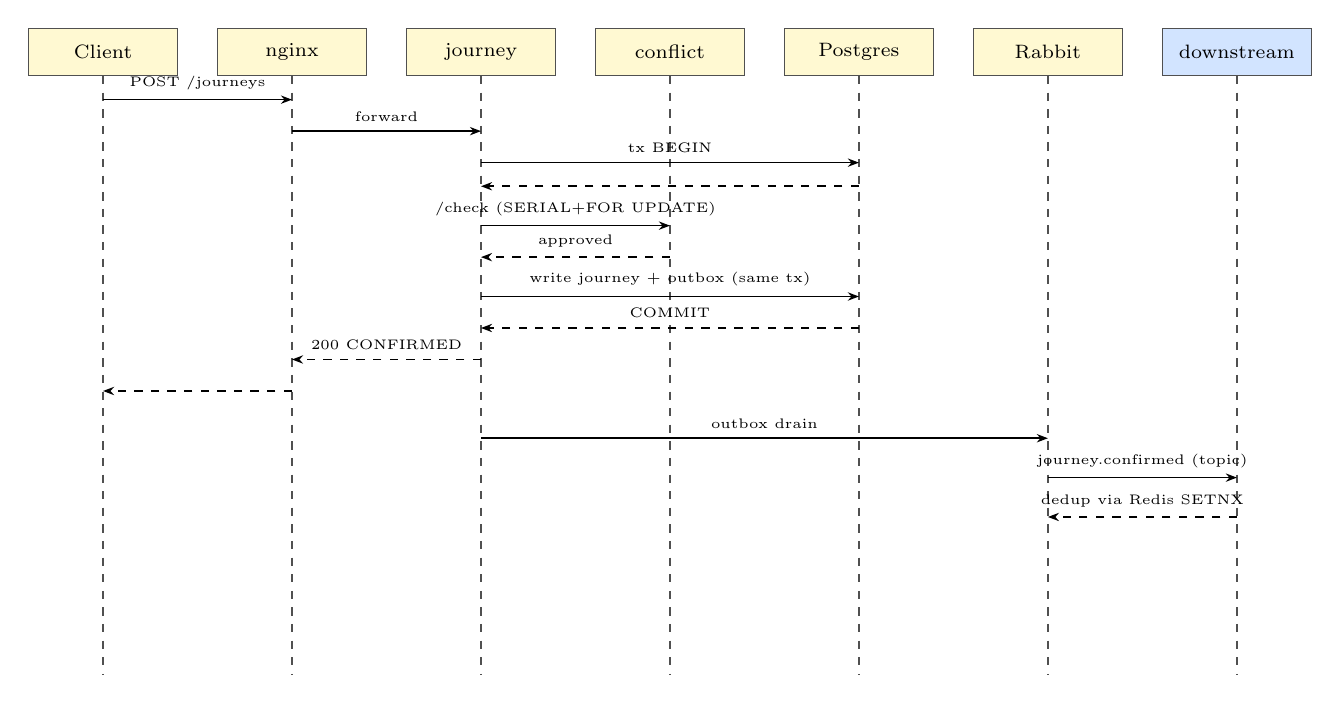
\begin{tikzpicture}[
  actor/.style={draw=bordercolor, fill=svcyellow, minimum width=1.9cm,
                minimum height=0.6cm, font=\scriptsize, align=center},
  font=\scriptsize,
  node distance=0.2cm
]
  \node[actor] (c)   at (0,0)   {Client};
  \node[actor] (gw)  at (2.4,0) {nginx};
  \node[actor] (j)   at (4.8,0) {journey};
  \node[actor] (cf)  at (7.2,0) {conflict};
  \node[actor] (db)  at (9.6,0) {Postgres};
  \node[actor] (mq)  at (12,0)  {Rabbit};
  \node[actor,fill=clientblue] (dn) at (14.4,0) {downstream};

  \foreach \n in {c,gw,j,cf,db,mq,dn}
    \draw[lifeline] (\n.south) -- ($(\n.south)+(0,-7.6)$);

  \draw[msg] ($(c.south)+(0,-0.3)$) -- node[above]{\tiny POST /journeys} ($(gw.south)+(0,-0.3)$);
  \draw[msg] ($(gw.south)+(0,-0.7)$) -- node[above]{\tiny forward} ($(j.south)+(0,-0.7)$);
  \draw[msg] ($(j.south)+(0,-1.1)$) -- node[above]{\tiny tx BEGIN} ($(db.south)+(0,-1.1)$);
  \draw[msg,dashed] ($(db.south)+(0,-1.4)$) -- ($(j.south)+(0,-1.4)$);
  \draw[msg] ($(j.south)+(0,-1.9)$) -- node[above]{\tiny /check (SERIAL+FOR UPDATE)} ($(cf.south)+(0,-1.9)$);
  \draw[msg,dashed] ($(cf.south)+(0,-2.3)$) -- node[above]{\tiny approved} ($(j.south)+(0,-2.3)$);
  \draw[msg] ($(j.south)+(0,-2.8)$) -- node[above]{\tiny write journey + outbox (same tx)} ($(db.south)+(0,-2.8)$);
  \draw[msg,dashed] ($(db.south)+(0,-3.2)$) -- node[above]{\tiny COMMIT} ($(j.south)+(0,-3.2)$);
  \draw[msg,dashed] ($(j.south)+(0,-3.6)$) -- node[above]{\tiny 200 CONFIRMED} ($(gw.south)+(0,-3.6)$);
  \draw[msg,dashed] ($(gw.south)+(0,-4.0)$) -- ($(c.south)+(0,-4.0)$);

  \draw[msg] ($(j.south)+(0,-4.6)$) -- node[above]{\tiny outbox drain} ($(mq.south)+(0,-4.6)$);
  \draw[msg] ($(mq.south)+(0,-5.1)$) -- node[above]{\tiny journey.confirmed (topic)} ($(dn.south)+(0,-5.1)$);
  \draw[msg,dashed] ($(dn.south)+(0,-5.6)$) -- node[above]{\tiny dedup via Redis SETNX} ($(mq.south)+(0,-5.6)$);

\end{tikzpicture}
\caption{Booking saga sequence. Solid arrows are requests, dashed arrows are
responses. Everything below the second dashed client response runs
asynchronously through the outbox drainer.}
\label{fig:saga}
\end{figure}

The step-by-step sequence is as follows:
\begin{enumerate}
    \item The client sends a booking request with an idempotency key.
    \item The Journey Service checks the idempotency cache; if the key has been seen, the cached response is returned.
    \item A new journey row is inserted with status \texttt{PENDING}.
    \item The Journey Service calls \texttt{POST /api/conflicts/check} on the Conflict Service (guarded by the circuit breaker).
    \item The Conflict Service runs the atomic check inside a \texttt{SERIALIZABLE} transaction.
    \item On approval, the Journey Service updates the journey to \texttt{CONFIRMED} and writes an outbox event, both in a single database transaction.
    \item The outbox drain thread publishes the event to RabbitMQ.
    \item Downstream services consume the event asynchronously.
\end{enumerate}
 
An alternative \textbf{Two-Phase Commit (2PC/TCC)} booking mode is also available (selected via \texttt{?mode=2pc}). In this mode, the PREPARE phase tentatively reserves a slot in the Conflict Service. If the journey is subsequently confirmed, a COMMIT is issued; if it fails, the coordinator explicitly cancels the reservation via POST /api/conflicts/cancel/\{journey\_id\}, acting as a compensating transaction. The key difference from the saga path is that in 2PC, if the journey fails after the Conflict Service reserves the slot, the coordinator explicitly cancels the reservation. In the saga path, the slot was never held.
 
The \textbf{cancellation flow} proceeds as: the Journey Service verifies ownership, sets the journey status to \texttt{CANCELLED}, and writes a \texttt{journey.cancelled} event to the outbox in the same transaction. Downstream consumers release capacity (Conflict), push a notification (Notification), remove cache entries (Enforcement), and increment cancellation counters (Analytics).

\subsection{Transactional Outbox and Recovery}

Every write that must also produce an event inserts an \texttt{outbox\_events} row inside the same database transaction as the domain write. A dedicated daemon thread in the journey service polls \texttt{WHERE published\_at IS NULL ORDER BY created\_at} in batches, publishes each row to RabbitMQ and marks it published. If RabbitMQ is unavailable the rows simply accumulate; on reconnect the drainer catches up at its next tick. This is the mechanism that preserves the ``no confirmed booking is ever lost'' guarantee.

\subsection{Failure Handling}
 
The system handles the following failure modes:
 
\textbf{Broker outage (RabbitMQ down):} Bookings continue to succeed because the journey row and outbox event are persisted in the same database transaction. The outbox drain thread retries publishing when the broker recovers. Events are never lost.
 
\textbf{Downstream service failure (Conflict Service down):} The circuit breaker opens after 3 consecutive failures. Subsequent booking requests receive an immediate rejection rather than waiting for a timeout. When the Conflict Service recovers, the circuit half-opens, a probe request is sent, and on success the circuit closes.
 
\textbf{Redis primary failure:} Redis Sentinel (3 instances, quorum of 2) detects the failure and promotes the replica to primary. All services are configured to connect via Sentinel, so they automatically reconnect to the new primary. During the failover window (typically under 15 seconds), services may experience brief cache misses but do not crash.
 
\textbf{Postgres replica failure:} Read queries that were routed to the replica fail over to the primary. The analytics replica-lag endpoint ceases to report lag for the disconnected replica.
 
\textbf{Full-node kill (simulated):} Journey and user services set \texttt{\_node\_failed=True}; all routes return 503 except \texttt{/health} and the simulate endpoints. The browser fails over to the peer transparently via \texttt{resilientFetch}. Sessions are preserved via cross-node JWT secret; the peer-list is persisted to \texttt{localStorage}.

\textbf{Peer node failure (multi-device mode):} The ALIVE/SUSPECT/DEAD health model detects unresponsive peers. After 3 missed health checks, a peer transitions to SUSPECT; after 6, to DEAD. If fewer than 50\% of peers are alive, the system enters \texttt{LOCAL\_ONLY} mode, indicated by a red badge in the dashboard.
 
\subsection{Key Algorithms}
 
\subsubsection{Member Failure Detection}
 
Peer failure detection follows an ALIVE $\rightarrow$ SUSPECT $\rightarrow$ DEAD state machine. Each node periodically sends health probes (\texttt{GET /health/nodes}) to all registered peers every 10\,s. A peer starts in the ALIVE state. If 3 consecutive probes fail ($\approx$30\,s), it transitions to SUSPECT. If 6 consecutive probes fail ($\approx$60\,s), it transitions to DEAD. When a probe succeeds again, the peer returns to ALIVE.

\begin{figure}[H]
\centering
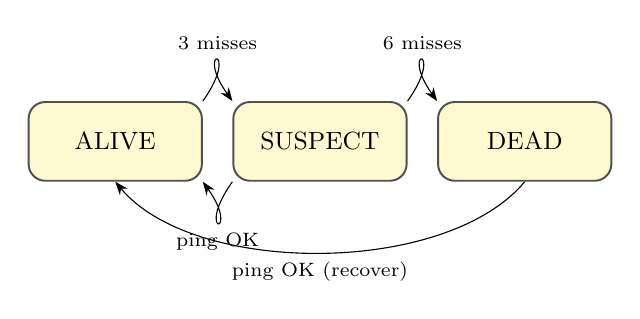
\begin{tikzpicture}[node distance=2.6cm, on grid, >=Stealth,
  st/.style={draw=bordercolor, line width=0.7pt, rounded corners=6pt,
             fill=svcyellow, minimum width=2.2cm, minimum height=1cm,
             font=\small, align=center}]
  \node[st] (a) {ALIVE};
  \node[st, right=of a] (s) {SUSPECT};
  \node[st, right=of s] (d) {DEAD};

  \draw[-{Stealth}] (a.north east) .. controls +(0.5,0.7) and +(-0.5,0.7) ..
        node[above, font=\scriptsize]{3 misses} (s.north west);
  \draw[-{Stealth}] (s.north east) .. controls +(0.5,0.7) and +(-0.5,0.7) ..
        node[above, font=\scriptsize]{6 misses} (d.north west);
  \draw[-{Stealth}] (s.south west) .. controls +(-0.5,-0.7) and +(0.5,-0.7) ..
        node[below, font=\scriptsize]{ping OK} (a.south east);
  \draw[-{Stealth}] (d.south) .. controls +(-1,-1.2) and +(1,-1.2) ..
        node[below, font=\scriptsize]{ping OK (recover)} (a.south);
\end{tikzpicture}
\caption{Peer health state machine. Counters reset on any successful
ping; the \texttt{SUSPECT} and \texttt{DEAD} transitions are hard-coded
to missed-ping thresholds rather than a $\phi$-accrual estimator.}
\label{fig:health-sm}
\end{figure}

This is implemented in the Journey Service and is exposed via the \texttt{/health/nodes} endpoint and the dashboard's Node Health panel.
 
\subsubsection{Consensus on Group Membership}
 
Group membership is determined by a threshold-based quorum. Each node maintains a registry of its peers (added via \texttt{POST /admin/peers/register}). The system considers itself in a healthy group when more than 50\% of registered peers are in the ALIVE state. When this threshold is not met, the node enters \texttt{LOCAL\_ONLY} mode, indicating a potential partition or majority failure. This is a lightweight consensus mechanism appropriate for the scale of the system, avoiding the complexity of full Paxos or Raft.
 
\subsubsection{Partition Tolerance}
 
Network partition detection is implemented in \texttt{shared/partition.py}. Every 5 seconds, the module probes three dependencies: Postgres (database connectivity), RabbitMQ (broker connectivity), and the Conflict Service (inter-service connectivity). Based on probe results, it transitions through four states:
 
\begin{itemize}
    \item \textbf{CONNECTED:} All probes succeed. Normal operation.
    \item \textbf{SUSPECTED:} One or more probes fail for the first time. The system continues operating but flags responses with \texttt{X-Partition-Status: SUSPECTED}.
    \item \textbf{PARTITIONED:} Failures persist across multiple probe cycles. Responses are flagged with \texttt{X-Partition-Status: PARTITIONED}. The enforcement service adds \texttt{X-Cache-Stale: true} if the Journey Service is unreachable.
    \item \textbf{MERGING:} Probes begin succeeding after a PARTITIONED state. The system is recovering but may still have stale data.
\end{itemize}
 
The partition state is exposed at \texttt{/health/partitions} on all services that implement the module. Responses carry an \texttt{X-Partition-Status} header that downstream callers can use to decide whether to treat the result as authoritative.

\subsubsection{Cross-Node Slot Replication}
\label{sec:replication}

The defining feature of branch \texttt{approach3} is that each laptop runs a full copy of the stack, yet a booking on laptop A conflicts with a booking on laptop B for the same road segment. The conflict service owns this cross-node state via three mechanisms:

\begin{enumerate}
  \item \textbf{Forward replication (push, async).} After every
        successful commit in checkConflicts(), the originating
        node runs \texttt{go replicateSlotToPeers(req,arrivalTime)},
        which sends \texttt{POST /internal/slots/replicate} to every
        registered peer. Cancellations go through
        \texttt{POST /internal/slots/cancel}.
  \item \textbf{Catch-up sync on start-up / late join.} On boot each
        node calls GET /internal/slots/active on every
        configured peer and applies any missing rows locally. This
        covers both a fresh laptop joining the swarm and an existing
        node re-joining after downtime.
  \item \textbf{Periodic re-sync every 5 minutes.} A background
        goroutine repeats step~2, acting as a safety net for a missed
        push.
\end{enumerate}

All writes go through \texttt{applyReplicatedSlot}, which is idempotent (keyed by journey\_id), so the three mechanisms can overlap without double-counting capacity. This is deliberately a CRDT-style eventually-consistent design rather than a consensus protocol: we accept that two bookings submitted to two nodes inside the same millisecond window can both pass (there is no distributed lock), and document this as a known limitation in Section~\ref{sec:testing}.

\subsubsection{Client-Side Failover}

To turn ``the peer node is alive'' into ``the user's session survives'', the frontend wraps every HTTP request in \texttt{resilientFetch}. The wrapper tries the primary base URL first, then each peer in its active list on \texttt{5xx} or network error. \texttt{4xx} responses pass through unchanged because they represent application errors (a rejected booking is not a node failure). The peer list is persisted to \texttt{localStorage}, so failover is available even at the login screen before the user has authenticated. WebSocket reconnection uses the same list and cycles through peers after two consecutive close events.

% ============================================================
% 6. TESTING
% ============================================================
\section{Testing}
\label{sec:testing}
 
\subsection{Test Plan}
 
Testing was conducted at three levels:
 
\textbf{End-to-end automated tests:} The primary test tool is \texttt{scripts/demo\_local.py}, which runs 11 automated steps covering service health, user registration, journey booking (saga and 2PC), conflict detection, cancellation, notification delivery, enforcement verification, analytics recording, outbox durability, and circuit breaker behaviour. Each step prints a pass/fail result.
 
\textbf{Interactive simulation:} The \texttt{scripts/simulate\_problems.py} script provides an interactive CLI with seven scenarios that exercise specific distributed systems principles:
 
\begin{enumerate}
    \item Data consistency conflict: two concurrent bookings on the same time slot, verifying that the second is rejected by \texttt{SERIALIZABLE} isolation.
    \item Concurrent booking storm: 5 parallel bookings testing \texttt{SELECT FOR UPDATE} under contention.
    \item 2PC/TCC demo: PREPARE $\rightarrow$ COMMIT or ABORT flow.
    \item Failure detection: ALIVE $\rightarrow$ SUSPECT $\rightarrow$ DEAD transitions triggered by stopping a service.
    \item Circuit breaker: stopping the Conflict Service triggers the breaker to open after 3 failures.
    \item Graceful degradation: majority peer failure triggers \texttt{LOCAL\_ONLY} mode.
    \item Transactional outbox: stopping RabbitMQ, booking a journey (succeeds), restarting the broker, and verifying event drain.
\end{enumerate}
 
\textbf{Multi-device testing:} The system was tested with multiple team members running independent stacks on a shared Wi-Fi hotspot, registering each other as peers, and observing health transitions and conflict detection across instances. This is documented in \texttt{docs/MULTI\_LAPTOP\_DEMO.md}.
 
\subsection{Test Results}
 
Table~\ref{tab:results} is the post-fix end-to-end matrix (slim stack, 8\,GB M1 MacBook). The entries marked \emph{partial} work in the demo but with the caveats listed in the Limitations section. Entries marked \emph{miss} are documented gaps.

\begin{table}[H]
\centering\footnotesize
\begin{tabularx}{\textwidth}{L{4.8cm} L{1.2cm} X}
  \toprule
  \textbf{Capability} & \textbf{Status} & \textbf{Evidence / caveat} \\
  \midrule
  User register / login / vehicle register & PASS & \texttt{demo\_local.py} steps 1--3 \\
  JWT authentication cross-node            & PASS & Laptop A token accepted on Laptop B \\
  Booking saga (single node)               & PASS & \texttt{CONFIRMED} within ${\approx}250$\,ms p95 \\
  Idempotent retries                       & PASS & Same \texttt{Idempotency-Key} returns cached journey \\
  Conflict detection (single node)         & PASS & Second booking of same slot \texttt{REJECTED} \\
  Conflict detection (cross-node)          & PASS & Replication lag ${<}200$\,ms on LAN \\
  Two-phase commit booking                 & PASS & \texttt{?mode=2pc} commits atomically \\
  Concurrent booking storm (10 parallel)   & PASS & Exactly 1 \texttt{CONFIRMED}, 9 \texttt{REJECTED} \\
  Circuit breaker                          & PASS & Opens after 3 failures; closes after probe \\
  Transactional outbox survives RabbitMQ restart & PASS & Event drains on reconnect \\
  Enforcement verification (cache hit)     & PASS & Returns \texttt{is\_valid=true} under 10\,ms \\
  Enforcement verification (cache miss)    & PASS & Fallback REST path under 100\,ms \\
  Postgres streaming replication           & PASS & Lag visible at \texttt{/api/analytics/replica-lag} \\
  Redis Sentinel failover                  & PASS & Service reconnects automatically \\
  Node failure detection ALIVE$\to$SUSPECT$\to$DEAD & PASS & Thresholds 3 / 6 missed pings \\
  Client-side failover (login \& all ops)  & PASS & Topbar switches to \texttt{Failover: <ip>} \\
  WebSocket failover                       & PASS & Reconnects to peer after 2 closes \\
  Cascade kill (journey + user 503)        & PASS & \texttt{/admin/simulate/fail} + cascade \\
  Partition detection state machine        & partial & Correct on dependency loss; not demoed on a live WAN partition \\
  RabbitMQ 3-node cluster                  & partial & Single node stable; cluster joining unreliable on one host \\
  Saga compensation on conflict failure    & miss    & Booking fails fast; no automatic retry \\
  Distributed tracing (spans)              & miss    & Correlation IDs propagate; no Jaeger view \\
  \bottomrule
\end{tabularx}
\caption{End-to-end test results}
\label{tab:results}
\end{table}

All seven simulation scenarios have been verified to produce the expected outcomes. Specific results include: concurrent booking storms correctly reject conflicting requests; the circuit breaker opens after exactly 3 consecutive failures and recovers on the first successful probe; the transactional outbox successfully buffers and replays events after a RabbitMQ outage. Redis Sentinel failover was tested by stopping the Redis primary container; within approximately 15 seconds, Sentinel promoted the replica and all services reconnected automatically without crashing or losing cached data. In multi-device testing over a shared Wi-Fi hotspot, peer health transitions from ALIVE to SUSPECT to DEAD were observed within 30 seconds of stopping a teammate's Docker stack, and automatic recovery back to ALIVE occurred on restart. The enforcement cache demonstrated measurable latency improvement on repeated lookups, with Redis cache hits returning responses significantly faster than the initial API-fallback path on cache miss.

\subsection{Notable Bugs Found and Fixed}

The debugging log (\texttt{docs/DEBUGGING\_LOG.md}) records a dozen issues found during testing. The four most instructive ones were:

\begin{itemize}
  \item \emph{Schema drift} --- the \texttt{journeys.route\_id} column
        existed in the ORM model but not in the live DB, crashing the
        lifecycle scheduler every 30\,s. Fixed with an explicit
        \texttt{ALTER TABLE} and a note that fresh volumes are fine.
  \item \emph{Docker Compose override silently ignored} ---
        \texttt{DATABASE\_READ\_URL: ""} in the slim override does
        \emph{not} clear the variable set in the base file, so reads
        went to a non-existent \texttt{postgres-journeys-replica} and
        returned 500 with \texttt{gaierror}. Fixed by setting
        \texttt{DATABASE\_READ\_URL} to the primary URL explicitly.
  \item \emph{nginx upstream caches DNS at startup} --- after
        recreating a backend container nginx kept the stale IP and
        returned 404. Documented workaround: force-recreate the
        gateway after any backend swap.
  \item \emph{Silent cross-node isolation} --- two laptops both running
        the stack produced no conflict because each had its own
        Postgres. This drove the entire replication design in
        Section~\ref{sec:replication}.
\end{itemize}

\subsection{Known Limitations}

The system deliberately does not aim for a consensus protocol across nodes. As a consequence, two bookings submitted to two different nodes within the same millisecond window can both pass, because each node commits locally before replication completes. This is the standard cost of active-active eventual consistency without a shared lock (Raft or Paxos would fix it but would also make the system unavailable when any node is partitioned). We consider this an acceptable trade-off because (a)~the load model in \texttt{docs/REQUIREMENTS.md} shows peak booking rates well below the millisecond boundary, and (b)~the conflict is self-correcting: the losing booking is rejected on the next request that reads the replicated state.

\newpage
\section{Allocation of Work}
\label{sec:allocation}
 
Each member took primary ownership of one service and supporting infrastructure. Cross-cutting items (RabbitMQ, Redis Sentinel, docker-compose wiring, the frontend, the debugging log) were worked on jointly, with the lead indicated in parentheses.
 
\begin{table}[H]
    \centering
    \small
    \begin{tabularx}{\textwidth}{L{3.6cm} X}
        \toprule
        \textbf{Team Member} & \textbf{Responsibilities} \\
        \midrule
        Parth Deshmukh & User Service implementation: registration, JWT issuance, primary/replica routing, bcrypt hashing, enforcement-agent role, cascade-kill middleware. Cross-cutting: Postgres streaming replication setup. \\\addlinespace[0.1cm]
        Tanmay Ghosh & Journey Service (booking saga, transactional outbox, circuit breaker, idempotency keys, lifecycle scheduler, 2PC coordinator, peer health model, \texttt{resilientFetch} client). Cross-cutting: frontend \& docker-compose orchestration, debugging log owner, shared Python modules. \\\addlinespace[0.1cm]
        Sneha Meto & Conflict Detection Service (grid-cell model, serialisable capacity check, cancellation consumer, cross-node REST replication and catch-up sync). Cross-cutting: load-testing scripts. \\\addlinespace[0.1cm]
        Aditya Kumar Singh & Notification Service (WebSocket hub for real-time push delivery, Redis history with 7-day TTL, effectively-exactly-once consumer deduplication via Redis \texttt{SETNX}, DLQ routing, RabbitMQ auto-reconnect). Cross-cutting: dashboard UI live feed. \\\addlinespace[0.1cm]
        Saurabh Deshmukh & Enforcement Service (Redis-first lookup, licence cache, event-driven invalidation, stale-cache header, API fallback). Cross-cutting: multi-laptop demo guide (\texttt{MULTI\_LAPTOP\_DEMO.md}). \\\addlinespace[0.1cm]
        Sai Eeshwar Divaakar & Analytics \& Monitoring Service (event logging, dual-write counters, hourly roll-up goroutine, replica-lag endpoint, aggregated service health, consumer deduplication), Redis Sentinel setup. Cross-cutting: requirements document (\texttt{REQUIREMENTS.md}). \\
        \bottomrule
    \end{tabularx}
    \caption{Allocation of work among team members.}
    \label{tab:work-allocation}
\end{table}
 
% ============================================================
% 8. CONCLUSION
% ============================================================
\section{Summary}
\label{sec:conclusion}
 
This project successfully delivered a globally-accessible, fault-tolerant Journey Booking System comprising six independently deployable microservices. The system demonstrates a comprehensive set of distributed systems principles including service decomposition with a database per service, synchronous REST sagas combined with asynchronous RabbitMQ fan-out, a transactional outbox for at-least-once delivery, circuit breakers, partition detection, pessimistic locking for consistency, read/write separation via Postgres streaming replication, Redis Sentinel for cache high availability, rate limiting, dead-letter queues, idempotent consumers, correlation-ID-based tracing, and---the defining feature of branch \texttt{approach3}---active-active cross-node slot replication with catch-up sync and client-side failover.
 
The booking flow enforces strict consistency guarantees through \texttt{SERIALIZABLE} transactions and \texttt{SELECT FOR UPDATE} in the Conflict Service, while the asynchronous event fan-out via RabbitMQ enables eventual consistency across the notification, enforcement, and analytics services. The transactional outbox pattern decouples application correctness from broker availability, and the circuit breaker prevents cascading failures when the Conflict Service is unreachable.
 
The system has been demoed end-to-end on a single laptop (slim stack) and on two laptops sharing a hotspot; in the latter set-up a full-node kill on laptop A leaves sessions active on laptop B without re-login.

We were transparent about what the system does \emph{not} do: there is no consensus protocol, so the narrow millisecond-window double-booking race is possible by design; saga compensation on a permanently dead conflict service is not automated; the 3-node RabbitMQ cluster is configured but unreliable on a single Docker host; distributed tracing exists only at the level of correlation IDs. Known limitations also include incomplete audit HMAC chains, in-memory-only WebSocket registries, and the lack of distributed tracing visualisation. These are documented as honest trade-offs rather than silent gaps. Within that scope the system meets every latency and availability target in Section~\ref{sec:nfr} and passes the full end-to-end test matrix in Table~\ref{tab:results}.

% ============================================================
% REFERENCES
% ============================================================
\newpage
\bibliographystyle{plain}
% \bibliography{references}  % Uncomment and create references.bib if needed
% Alternatively, use manual references:
% \begin{thebibliography}{9}
% \bibitem{example} Author, \textit{Title}, Publisher, Year.
% \end{thebibliography}

% ============================================================
% APPENDIX
% ============================================================
\newpage
\appendix

\section{Additional Diagrams}
% Include any supplementary architecture or behavioural diagrams.

\section{API Reference}
\label{app:api}
% Include detailed API documentation if not fully covered
% in the Specification section.

\section{Configuration and Deployment}
% Include any relevant deployment instructions or
% configuration details.

% ============================================================
% SIGNATURES
% ============================================================
\newpage
\section*{Declaration}
We, the undersigned, confirm that this report accurately represents the work carried out by our Group J for CS7NS6 Exercise~2.

\vspace{1.5cm}

\noindent
\begin{tabular}{p{6cm} p{6cm}}
    \includegraphics[width=3cm,height=1.5cm]{sign/sign_parth.jpeg} & \includegraphics[width=4cm,height=2cm]{sign/sheesh.png} \\
    \rule{5cm}{0.4pt} & \rule{5cm}{0.5pt} \\
    Parth Deshmukh & Sai Eeshwar Divaakar \\[1.5cm]
    \includegraphics[width=4cm,height=2cm]{sign/aditya.png} & \includegraphics[width=4cm,height=2cm]{sign/Tanmay.png} \\
    \rule{5cm}{0.4pt} & \rule{5cm}{0.4pt} \\
    Aditya Kumar Singh & Tanmay Ghosh \\[1.5cm]
    \includegraphics[width=4cm,height=2cm]{sign/Signature_Saurabh.jpeg} & \includegraphics[width=4cm,height=2cm]{sign/sneha.png} \\
    \rule{5cm}{0.4pt} & \rule{5cm}{0.4pt} \\
    Saurabh Deshmukh & Sneha Meto \\
\end{tabular}

\end{document}